\documentclass[a4paper, 11pt]{article}
\usepackage{amsfonts}
\usepackage{systeme}
\usepackage{graphicx}
\usepackage[left=2cm, top=3cm, text={17cm, 24cm}]{geometry}

\begin{document}
\section*{\huge{Výstupní zpráva INC}}
Jméno: Artur Sultanov \\
Login: xsulta01
\section{Architektura navrženého obvodu (na úrovni RTL)}
\subsection{Schéma obvodu}
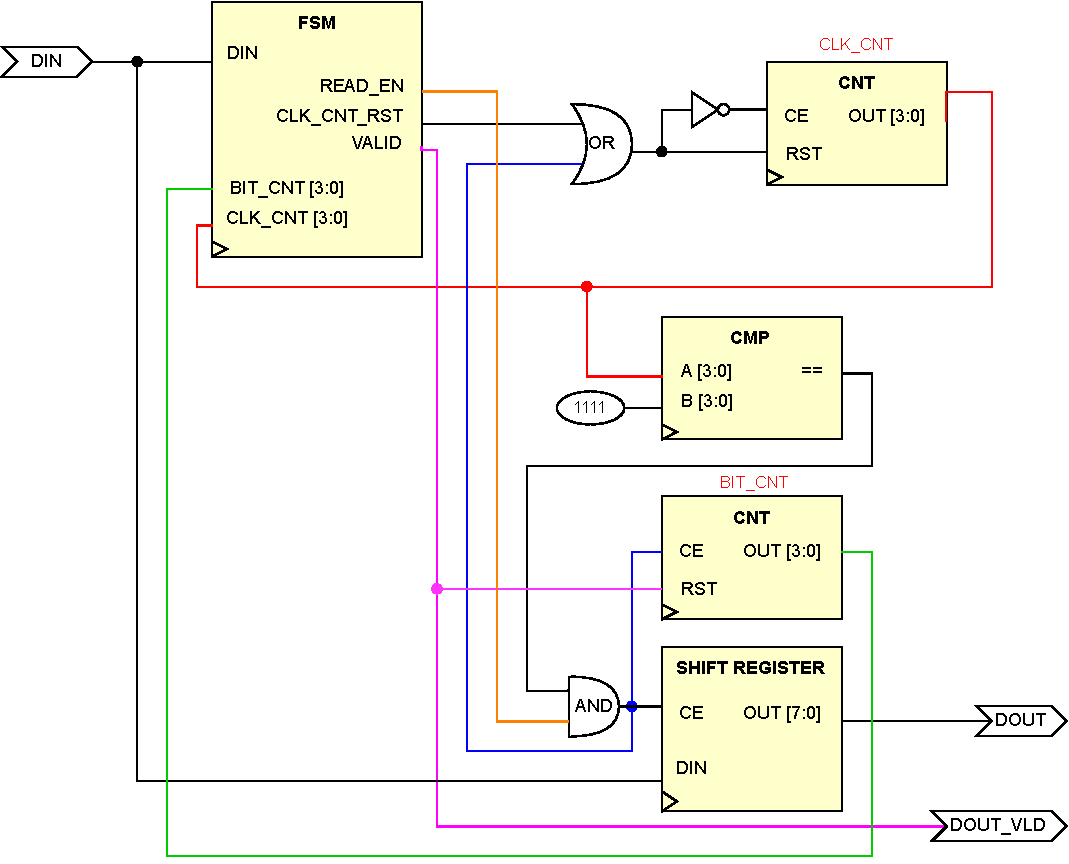
\includegraphics[width=\textwidth,height=\textheight,keepaspectratio]{INC_RTL.pdf}
\subsection{Popis funkce}
Obvod slouží ke čtení datových slov po asynchronní sériové lince (UART\_RX). Obvod používá FSM pro řízení chodu celého obvodu, schéma je zobrazeno níže.
V obvodu jsou dva čítače. Čítač CLK\_CNT počítá hodinové cykly a může fungovat ve dvou režimech, které závislí na výstupe READ\_EN FSM. Při READ\_EN = '0' čítač běží v "neomezeném" režimu. Při READ\_EN = '1' čítač běží v "omezeném" režimu a restartujte každý 16 cyklu, toto je zaručeno comparatorem CMP. Pro výstup je použit shift register, který po 16 cyklech čte hodnotu ze vstupu DIN, toto je také zaručeno comparatorem CMP.

\newpage
\section{Návrh automatu (Finite State Machine)}
\subsection{Schéma automatu}
Legenda
\begin{itemize}
  \item Stavy automatu: WAIT\_FOR\_START, WAIT\_FOR\_MID\_BIT, CLK\_CNT\_RST, READING\_DATA, WAIT\_FOR\_STOP, VALIDATING.
  \item Vstupní signály: DIN, BIT\_CNT, CLK\_CNT.
  \item Moorovy výstupy: READ\_EN, CLK\_CNT\_RST, VALID.
\end{itemize}
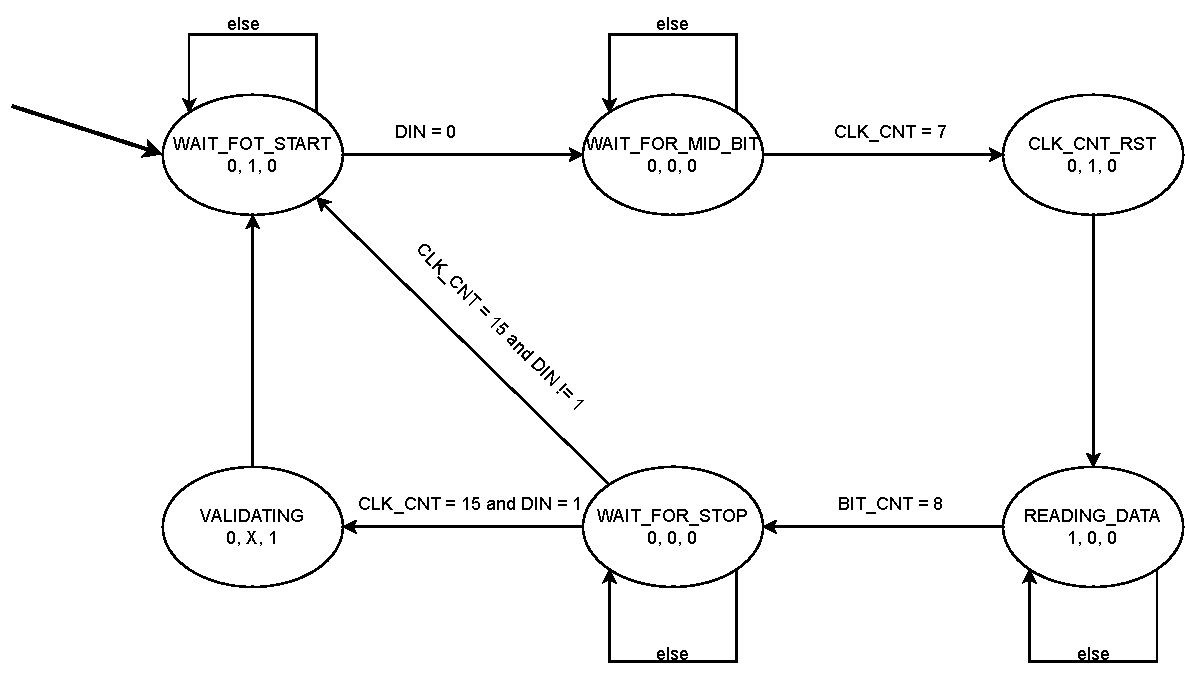
\includegraphics[width=\textwidth,height=\textheight,keepaspectratio]{INC_FSM.pdf}
\subsection{Popis funkce}
Automat začíná ve stavu WAIT\_FOR\_START a čeká na START BIT. Při změně {DIN = 0} (t.j. START BITů) automat přejde do WAIT\_FOR\_MID\_BIT. Ve stavu WAIT\_FOR\_MID\_BIT se začínají počítat hodinové cykly (CLK\_CNT). Kdy CLK\_CNT = 7 automat přejde do stavu CLK\_CNT\_RST. Ve stavu CLK\_CNT\_RST se nacházíme v MIDBITů START BITů, restartuje čítač CLK\_CNT, a automat přejde do stavu READING\_DATA. Ve stavu READING\_DATA se začínají počítat přenesený bity (BIT\_CNT) a znovu začínají se počítat hodinové cykly  (CLK\_CNT v "omezeném" režimu, t.j. čítač se restartuje každý 16 cyklů). Kdy BIT\_CNT = 8 automat přejde do stavu WAIT\_FOR\_STOP. Ve stavu WAIT\_FOR\_STOP automat se čeká 16 cyklů CLK. Po 16 cyklů: jestli vtupní signál DIN = 1 (t.j. STOP BITů) automat přijde do stavu VALIDATING; jestli vtupní signál DIN se nerovná '1' automat přijde do stavu WAIT\_FOR\_START. Ve stavu VALIDATING se zapíše na výstup, že  hodnota v shift registru je validní a automat přejde do stavu WAIT\_FOR\_START.
\newpage
\section{Snímek obrazovky ze simulací}
\begin{center}
  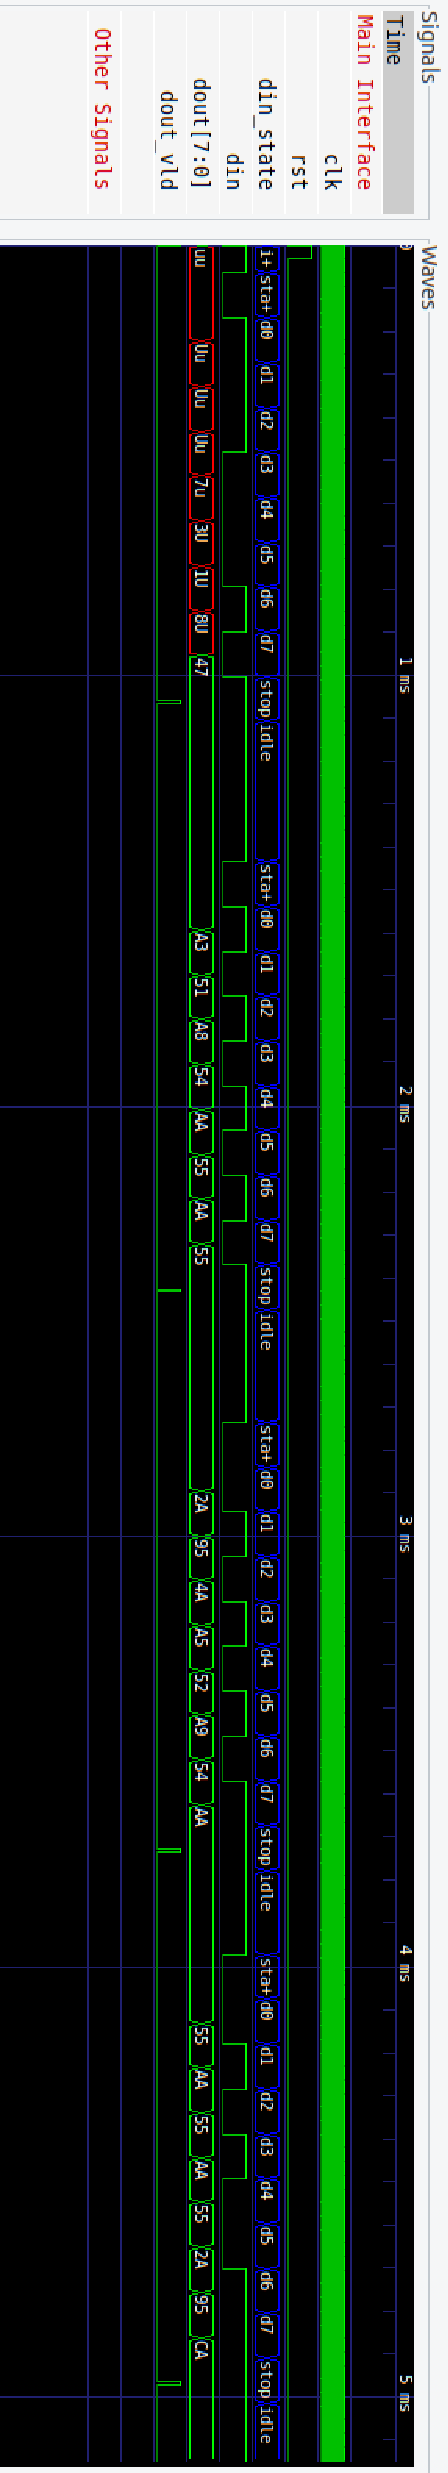
\includegraphics[width=0.4\textheight,height=1.475\textwidth]{wave.pdf}
\end{center}
\end{document}